% Options for packages loaded elsewhere
\PassOptionsToPackage{unicode}{hyperref}
\PassOptionsToPackage{hyphens}{url}
\PassOptionsToPackage{dvipsnames,svgnames,x11names}{xcolor}
%
\documentclass[
  12pt,
]{interact}

\usepackage{amsmath,amssymb}
\usepackage{setspace}
\usepackage{iftex}
\ifPDFTeX
  \usepackage[T1]{fontenc}
  \usepackage[utf8]{inputenc}
  \usepackage{textcomp} % provide euro and other symbols
\else % if luatex or xetex
  \usepackage{unicode-math}
  \defaultfontfeatures{Scale=MatchLowercase}
  \defaultfontfeatures[\rmfamily]{Ligatures=TeX,Scale=1}
\fi
\usepackage{lmodern}
\ifPDFTeX\else  
    % xetex/luatex font selection
\fi
% Use upquote if available, for straight quotes in verbatim environments
\IfFileExists{upquote.sty}{\usepackage{upquote}}{}
\IfFileExists{microtype.sty}{% use microtype if available
  \usepackage[]{microtype}
  \UseMicrotypeSet[protrusion]{basicmath} % disable protrusion for tt fonts
}{}
\makeatletter
\@ifundefined{KOMAClassName}{% if non-KOMA class
  \IfFileExists{parskip.sty}{%
    \usepackage{parskip}
  }{% else
    \setlength{\parindent}{0pt}
    \setlength{\parskip}{6pt plus 2pt minus 1pt}}
}{% if KOMA class
  \KOMAoptions{parskip=half}}
\makeatother
\usepackage{xcolor}
\setlength{\emergencystretch}{3em} % prevent overfull lines
\setcounter{secnumdepth}{5}
% Make \paragraph and \subparagraph free-standing
\makeatletter
\ifx\paragraph\undefined\else
  \let\oldparagraph\paragraph
  \renewcommand{\paragraph}{
    \@ifstar
      \xxxParagraphStar
      \xxxParagraphNoStar
  }
  \newcommand{\xxxParagraphStar}[1]{\oldparagraph*{#1}\mbox{}}
  \newcommand{\xxxParagraphNoStar}[1]{\oldparagraph{#1}\mbox{}}
\fi
\ifx\subparagraph\undefined\else
  \let\oldsubparagraph\subparagraph
  \renewcommand{\subparagraph}{
    \@ifstar
      \xxxSubParagraphStar
      \xxxSubParagraphNoStar
  }
  \newcommand{\xxxSubParagraphStar}[1]{\oldsubparagraph*{#1}\mbox{}}
  \newcommand{\xxxSubParagraphNoStar}[1]{\oldsubparagraph{#1}\mbox{}}
\fi
\makeatother


\providecommand{\tightlist}{%
  \setlength{\itemsep}{0pt}\setlength{\parskip}{0pt}}\usepackage{longtable,booktabs,array}
\usepackage{calc} % for calculating minipage widths
% Correct order of tables after \paragraph or \subparagraph
\usepackage{etoolbox}
\makeatletter
\patchcmd\longtable{\par}{\if@noskipsec\mbox{}\fi\par}{}{}
\makeatother
% Allow footnotes in longtable head/foot
\IfFileExists{footnotehyper.sty}{\usepackage{footnotehyper}}{\usepackage{footnote}}
\makesavenoteenv{longtable}
\usepackage{graphicx}
\makeatletter
\newsavebox\pandoc@box
\newcommand*\pandocbounded[1]{% scales image to fit in text height/width
  \sbox\pandoc@box{#1}%
  \Gscale@div\@tempa{\textheight}{\dimexpr\ht\pandoc@box+\dp\pandoc@box\relax}%
  \Gscale@div\@tempb{\linewidth}{\wd\pandoc@box}%
  \ifdim\@tempb\p@<\@tempa\p@\let\@tempa\@tempb\fi% select the smaller of both
  \ifdim\@tempa\p@<\p@\scalebox{\@tempa}{\usebox\pandoc@box}%
  \else\usebox{\pandoc@box}%
  \fi%
}
% Set default figure placement to htbp
\def\fps@figure{htbp}
\makeatother

\usepackage{booktabs}
\usepackage{longtable}
\usepackage{array}
\usepackage{multirow}
\usepackage{wrapfig}
\usepackage{float}
\usepackage{colortbl}
\usepackage{pdflscape}
\usepackage{tabu}
\usepackage{threeparttable}
\usepackage{threeparttablex}
\usepackage[normalem]{ulem}
\usepackage{makecell}
\usepackage{xcolor}
\usepackage{orcidlink}
\makeatletter
\@ifpackageloaded{caption}{}{\usepackage{caption}}
\AtBeginDocument{%
\ifdefined\contentsname
  \renewcommand*\contentsname{Table of contents}
\else
  \newcommand\contentsname{Table of contents}
\fi
\ifdefined\listfigurename
  \renewcommand*\listfigurename{List of Figures}
\else
  \newcommand\listfigurename{List of Figures}
\fi
\ifdefined\listtablename
  \renewcommand*\listtablename{List of Tables}
\else
  \newcommand\listtablename{List of Tables}
\fi
\ifdefined\figurename
  \renewcommand*\figurename{Figure}
\else
  \newcommand\figurename{Figure}
\fi
\ifdefined\tablename
  \renewcommand*\tablename{Table}
\else
  \newcommand\tablename{Table}
\fi
}
\@ifpackageloaded{float}{}{\usepackage{float}}
\floatstyle{ruled}
\@ifundefined{c@chapter}{\newfloat{codelisting}{h}{lop}}{\newfloat{codelisting}{h}{lop}[chapter]}
\floatname{codelisting}{Listing}
\newcommand*\listoflistings{\listof{codelisting}{List of Listings}}
\makeatother
\makeatletter
\makeatother
\makeatletter
\@ifpackageloaded{caption}{}{\usepackage{caption}}
\@ifpackageloaded{subcaption}{}{\usepackage{subcaption}}
\makeatother

\usepackage[]{natbib}
\bibliographystyle{plainnat}
\usepackage{bookmark}

\IfFileExists{xurl.sty}{\usepackage{xurl}}{} % add URL line breaks if available
\urlstyle{same} % disable monospaced font for URLs
\hypersetup{
  pdftitle={Inside Out: Externalizing Assumptions in Data Analysis as Validation Checks},
  pdfauthor={H. Sherry Zhang; Roger D. Peng},
  colorlinks=true,
  linkcolor={blue},
  filecolor={Maroon},
  citecolor={Blue},
  urlcolor={Blue},
  pdfcreator={LaTeX via pandoc}}


\title{Inside Out: Externalizing Assumptions in Data Analysis as
Validation Checks}
\author{H. Sherry Zhang$\textsuperscript{1}$, Roger D.
Peng$\textsuperscript{1}$}

\thanks{CONTACT: H. Sherry
Zhang. Email: \href{mailto:huize.zhang@austin.utexas.edu}{\nolinkurl{huize.zhang@austin.utexas.edu}}. Roger
D.
Peng. Email: \href{mailto:roger.peng@austin.utexas.edu}{\nolinkurl{roger.peng@austin.utexas.edu}}. }
\begin{document}
\captionsetup{labelsep=space}
\maketitle
\textsuperscript{1} Department of Statistics and Data
Sciences, University of Texas at Austin, Texas, United States
\begin{abstract}
In data analysis, unexpected results often prompt researchers to revisit
their procedures to identify potential issues. While some researchers
may struggle to identify the root causes, experienced researchers can
often quickly diagnose problems by checking a few key assumptions. These
checked assumptions, or expectations, are typically informal, difficult
to trace, and rarely discussed in publications. In this paper, we
introduce the term \emph{analysis validation checks} to formalize and
externalize these informal assumptions. We then introduce a procedure to
identify a subset of checks that best predict the occurrence of
unexpected outcomes, based on simulations of the original data. The
checks are evaluated in terms of accuracy, determined by binary
classification metrics, and redundancy, which measures the shared
information among checks using mutual information. We demonstrate this
approach with a toy example using step count data and a generalized
linear model example examining the effect of particulate matter air
pollution on daily mortality.
\end{abstract}


\setstretch{1.15}
\section{Introduction}\label{introduction}

In data analysis, analysts often rely on their prior knowledge or domain
expertise to form expectations and assess whether results align with
them. When results deviate from these expectations, experienced analysts
check assumptions made about the data and during the analysis, but often
do so without discussing the underlying reasoning in the publications.
While publication of analysis code and data is now a common a
requirement for the sake of reproducibility
\citep{peng2011reproducible}, the published code alone is often
insufficient for understanding the thought process behind an analysis.
Code corresponding to published analyses often reflect the final
decisions made about analysis and do not reveal the decisions or
assumptions made about the data during the analysis. Thus, a reader
looking at published code can often be left with many questions about
why certain choices were made.

We might gain insight into analysts' thought processes by speaking with
them directly or watching them work via screencast videos they produce,
such as, TidyTuesday screencast videos or think-aloud type studies
\citep[e.g.][]{gu2024data}. However, direct observation of analysis is
not scalable and may not always be feasible; creating educational
screencast videos requires significant effort from the analysts.
Ideally, there could be a way to explicitly communciate these throught
processes in the data analysis to others. Even better, if these
expectations were machine-readable, we could analyze them and learn from
the analysis itself. For example, we could answer questions about
whether the checks also apply to other researchers analyzing new data in
the same context, whether they reflect common practices in the field, or
whether they are specific to the data or analysis at hand. Externalizing
these thought processes is a practice that has potential to improve the
trustworthiness of the analyses \citep{yu2024veridical} in general and
the trustworthiness of subsequent products, such as machine learning
models, that may be built on such analyses. Developing an approach to
reveal some of this process without requiring a reader to essentially
reconstruct the analysis process from the raw data would provide an
improved basis for trusting an analysis result
\citep{peng2021reproducible}.

In this paper, we conceptualize these inexplicit expectations as
\emph{analysis validation checks}, which allows us to examine the
assumptions made about the data during an analysis. We then introduce a
procedure to identify the subset of checks that best predict the
occurrence of unexpected outcomes. The procedure, based on simulations
of the original data, compares the accuracy and redundancy of different
combinations of analysis validation checks. Accuracy is determined using
binary classification metrics (precision and recall) from a logic
regression model \citep{ruczinski_logic_2003}, while redundancy is
measured using mutual information. The proposed workflow offers a
numerical guarantee that the analysis will produce the expected results,
assuming the assumptions about the data generating mechanism hold.

The rest of the paper is organized as follows:
Section~\ref{sec-lit-review} reviews the concepts of diagnosing
unexpected outcomes and general data quality checks.
Section~\ref{sec-plan} introduces the concept of analysis validation
checks, illustrated with a toy example based on step count data.
Section~\ref{sec-method} describes the procedure that selects the best
subset of checks for understanding the occurrence of unexpected
outcomes. Section~\ref{sec-pm10-mortality} applies this procedure to a
larger example that estimates the effect of particulate matter air
pollution on daily mortality. Section~\ref{sec-discussion} summarises
the paper and discusses a few key considerations.

\section{Related Work}\label{sec-lit-review}

\subsection{Diagnosing unexpected outcomes in data
analysis}\label{diagnosing-unexpected-outcomes-in-data-analysis}

The concept of framing data analysis as a sense-making process was
originally presented by \citet{grolemund_cognitive_2014} based on
seminal work by \citet{wild1999statistical}. Key to any sense-making
process is a model for the world (i.e.~expectations for what we might
observe) and observed data with which we can compare our expectations.
If there is a significant deviation between what we observe and our
expectations, then a data analysis must determine what is causing that
deviation. A naive approach would be to update our model for the world
to match the data, under the assumption that the initial expectation was
incorrect. However, experienced analysts know that the reality can be
more nuanced than that, with errors occurring in data collection or data
processing that can have an impact on final results.

The skill of diagnosing unexpected data analysis results is not one that
has received significant attention in the statistics literature. While
the concept of diagnosis is often embedded in model checking or data
visualization techniques, systematic approaches to identifying the root
cause of a general unexpected analysis result are typically not
presented \citep{peng2022perspective}. Furthermore, if interesting
information is discovered through model checking or data visualization,
there is no formal way to document such discoveries for the next analyst
to consider. \citet{peng_diagnosing_2021} proposed a series of exercises
for training students in data analysis to diagnose different kinds of
analysis problems such as coding errors or outliers. They provide a
systematic approach involving working backwards from the analysis result
to identify potential causes. There are parallels here to the concept of
debugging and testing in software engineering
\citep{donoghue2021teaching}. For example, \citet{li2019towards} found
that experienced engineers were generally able to identify problems in
code faster than novices, and that the ability to debug code required
knowledge that cut across different domains.

If it is true that the speed with which data analysts can identify
problems with an analysis is related to their experience working with a
given type of data, then there is perhaps room to improve the analytic
process by externalizing the aspects that an analyst learns through
experience. That way, inexperienced analysts could examine the thought
process of an experienced analyst and learn to identify factors that can
cause unexpected results to occur.

\subsection{Data analysis checks}\label{data-analysis-checks}

The concept of data quality has been studied in the literature, with
earlier work focusing on defining frameworks -- such as dimensions,
attributes, and measures -- to improve data quality in database and
information systems
\citep{wang1996beyond, batini2009methodologies, 6204995, woodall2014classification, cai2015challenges, 8642813}.
More recently, data validation has been incorporated into frameworks
like Google TensorFlow \citep{polyzotis2019data} to ensure the quality
of data for training machine learning models, as well as for supporting
business decision-making \citep{schelter2018automating}. With the
increasing availability of open data in scientific research, the users
of the data are often not the original data collector and may not be
aware of all the details or nuances of the data. This encourages
researchers to conduct data quality checks before beginning the analytic
process, helping to avoid unexpected discoveries later on. In R,
packages like \texttt{skimr} \citep{skimr} and \texttt{dataMaid}
\citep{dataMaid} provide basic data screening and data quality reports,
while packages such as \texttt{assertr} \citep{assertr},
\texttt{validate} \citep{validate}, and \texttt{pointblank}
\citep{pointblank} focuse on providing infustructures that allow users
to define customized data quality checks.

The literature on data quality typically focuses on the intrinsic or
inherent quality of the data themselves, rather than the data's
relationship to any specific data analysis. So for example, if a column
in a data table is expecting numerical data, but we observe a character
value in one of the entries, then that occurrence would trigger some
sort of data quality check. This type of quality check can be triggered
without any knowledge of what the data will ultimately be used for.
However, for a given analysis, we may require specific aspects of the
data to be true because they affect the result being computed.
Conversely, certain types of poor quality data may have little impact on
the ultimate result of an analysis (e.g.~data that are missing
completely at random). Defining data quality in terms of what may affect
a specific analysis outcome or result has the potential to open new
avenues for defining data checks and for building algorithms for
optimizing the collection of checks defined for a specific analysis.

\section{Analysis validation checks}\label{sec-plan}

Analysis validation checks are assumptions made by the analysts during
the analysis, framed as explicit checks that return a binary TRUE or
FALSE value based on the data. Inspired by the concept of data
validation checks \citep{validate}, which are designed to ensure that
datasets meet expected quality before the analysis begins, analysis
validation checks reverse the approach: they validate the assumptions
about the data necessary for the analysis to produce the \emph{expected
results}, as defined by the analyst. The focus on expected results
allows analysis validation checks to encompass a wide range of checks,
such as data quality, variable distributions and outliers, bivariate and
multivariate relationships, and contextual information relevant to the
analysis.

Our proposed analysis validation checks provide insights into an
analyst's thought process and offer the following benefits:

\begin{enumerate}
\def\labelenumi{\arabic{enumi}.}
\tightlist
\item
  Serve as clear checkpoints to support the replication or application
  of methods to (new) data by programmatically communicating the
  requirements or assumptions made of the data;
\item
  Align assumptions among researchers from different domain backgrounds
  who may have different expectations about the data;
\item
  Improve analysis transparency, reproducibility, and trustworthiness by
  externalizing a key part of the analysis process; and
\item
  Quantify the effectiveness of analysis checks for predicting the
  expected outcome (see Section~\ref{sec-method});
\end{enumerate}

In addition to the above benefits, the development and publication of
analysis checks have the potential to help students, inexperienced
analysts, and junior researchers develop the skills needed to diagnose
unexpected analysis results for a given type of data because the
assumptions made about the data are made transparent. The analysis
checks can serve as a basis for new analysts to have conversations about
the data they are analyzing and to develop a better understanding of the
potential data generation process.

\subsection{A Toy Example}\label{sec-toy}

Consider a 30-day step count experiment in a public health setting.
Subjects are instructed to walk at least 8,000 steps each day, with an
expected average of 9,000 steps, tracked by a step counter app. With
data of this nature, we may expect there to be occasional ``low'' days
due to factors such as unfavorable weather conditions limiting outdoor
activities. We may also expect ``high'' days recorded after an outdoor
activities or intense workout. Given the requirements of the study, we
form our expectation as follows:

\begin{quote}
Expectation: The average step count of a given subject is between
\([8,500, 9,500]\)
\end{quote}

To diagnose potential reasons why this expectation might fail, we can
establish a few analysis validation checks in anticipation of seeing the
data. For example, we can check the quantile of the step count, if more
than a third of the days fall below 8,000, or more than a third exceed
10,000 steps, this could indicate an excess of low-count or high-count
days. Similarly, we may may expect the standard deviation of the step
count not to be overly large. These considerations yield the following
three analysis validation checks that \emph{fail} when:

\begin{itemize}
\tightlist
\item
  Check 1: the 60\% quantile of the observed step counts is greater than
  10,000
\item
  Check 2: the 40\% quantile of the observed step counts is less than
  8,000, and
\item
  Check 3: the standard deviation of the observed step counts exceeds
  2,500.
\end{itemize}

The cutoff values for these checks would presumably be chosen based on
prior experience with these kinds of data, but could also be optimized
using the method presented in the next section.

To simulate this data, three normal distributions are used for the daily
step counts: \(\mathcal{N}(6,000, 200)\) for low days,
\(\mathcal{N}(12,000, 200)\) for high days, and
\(\mathcal{N}(9,000, 300)\) for typical days. The number of low and high
days can be simulated from a Poisson distribution with \(\lambda = 8\).
Figure~\ref{fig-step-count} displays average step count across 300
simulated 30-day periods.

\phantomsection\label{cell-fig-step-count}
\begin{figure}[H]

\centering{

\pandocbounded{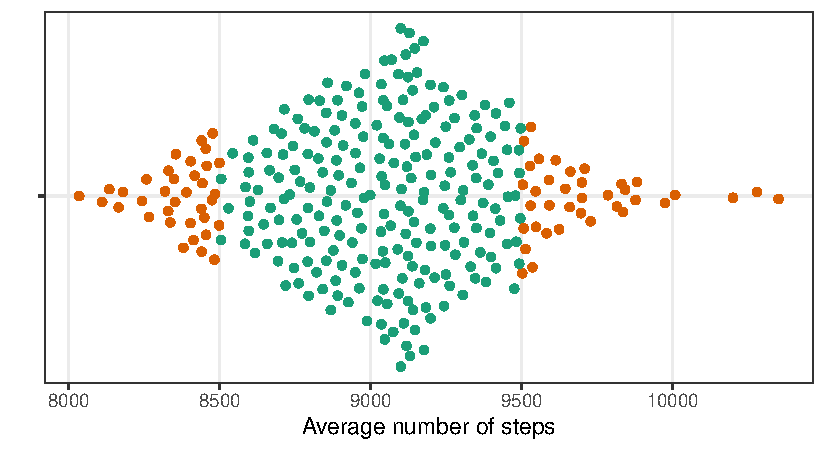
\includegraphics[keepaspectratio]{index_files/figure-pdf/fig-step-count-1.pdf}}

}

\caption{\label{fig-step-count}Beeswarm plot of average step counts
across 300 simulated 30-day periods. Each point represents the average
step count from one simulation. Similar to a boxplot or violin plot, the
beeswarm plot also displays the distribution of each individual data
point. The orange points indicate instances where the average step count
fails outside the {[}8,500, 9,500{]} interval, representing an
unexpected outcome in this scenario.}

\end{figure}%

\section{Method}\label{sec-method}

While some checks may be crucial and directly indicate an unexpected
outcome, others may be tangential to the problem at hand and not
indicate a root cause of an unexpected outcome. In this section, we
propose a procedure to measure the effectiveness of checks that, when
combined using logical operators, contribute to an unexpected outcome. A
small set of independent checks is considered effective if it translates
to unexpected outcomes.

The approach relies on the use of simulated datasets that are generated
based on the analyst's knowledge and assumptions about the data
generation mechanism. Datasets are simulated to have the same structure
and characteristics of the observed data that will be analyzed at some
point in the future. For each simulated dataset, we can apply a
collection of analysis validation checks to the dataset and record which
ones were TRUE and which were FALSE. We can also compute the outcome of
the analysis to see whether the outcome is unexpected in a given
simulated datsets. We can then generate many datasets, each time
applying the analysis validation checks and computing the outcome. After
generating many datasets, we can relate the patterns in the analysis
validation checks to the likely that the outcome will be unexpected in a
given dataset. Figure~\ref{fig-metric-calc} provides an overview of the
process.

\phantomsection\label{cell-fig-metric-calc}
\begin{figure}[H]

\centering{

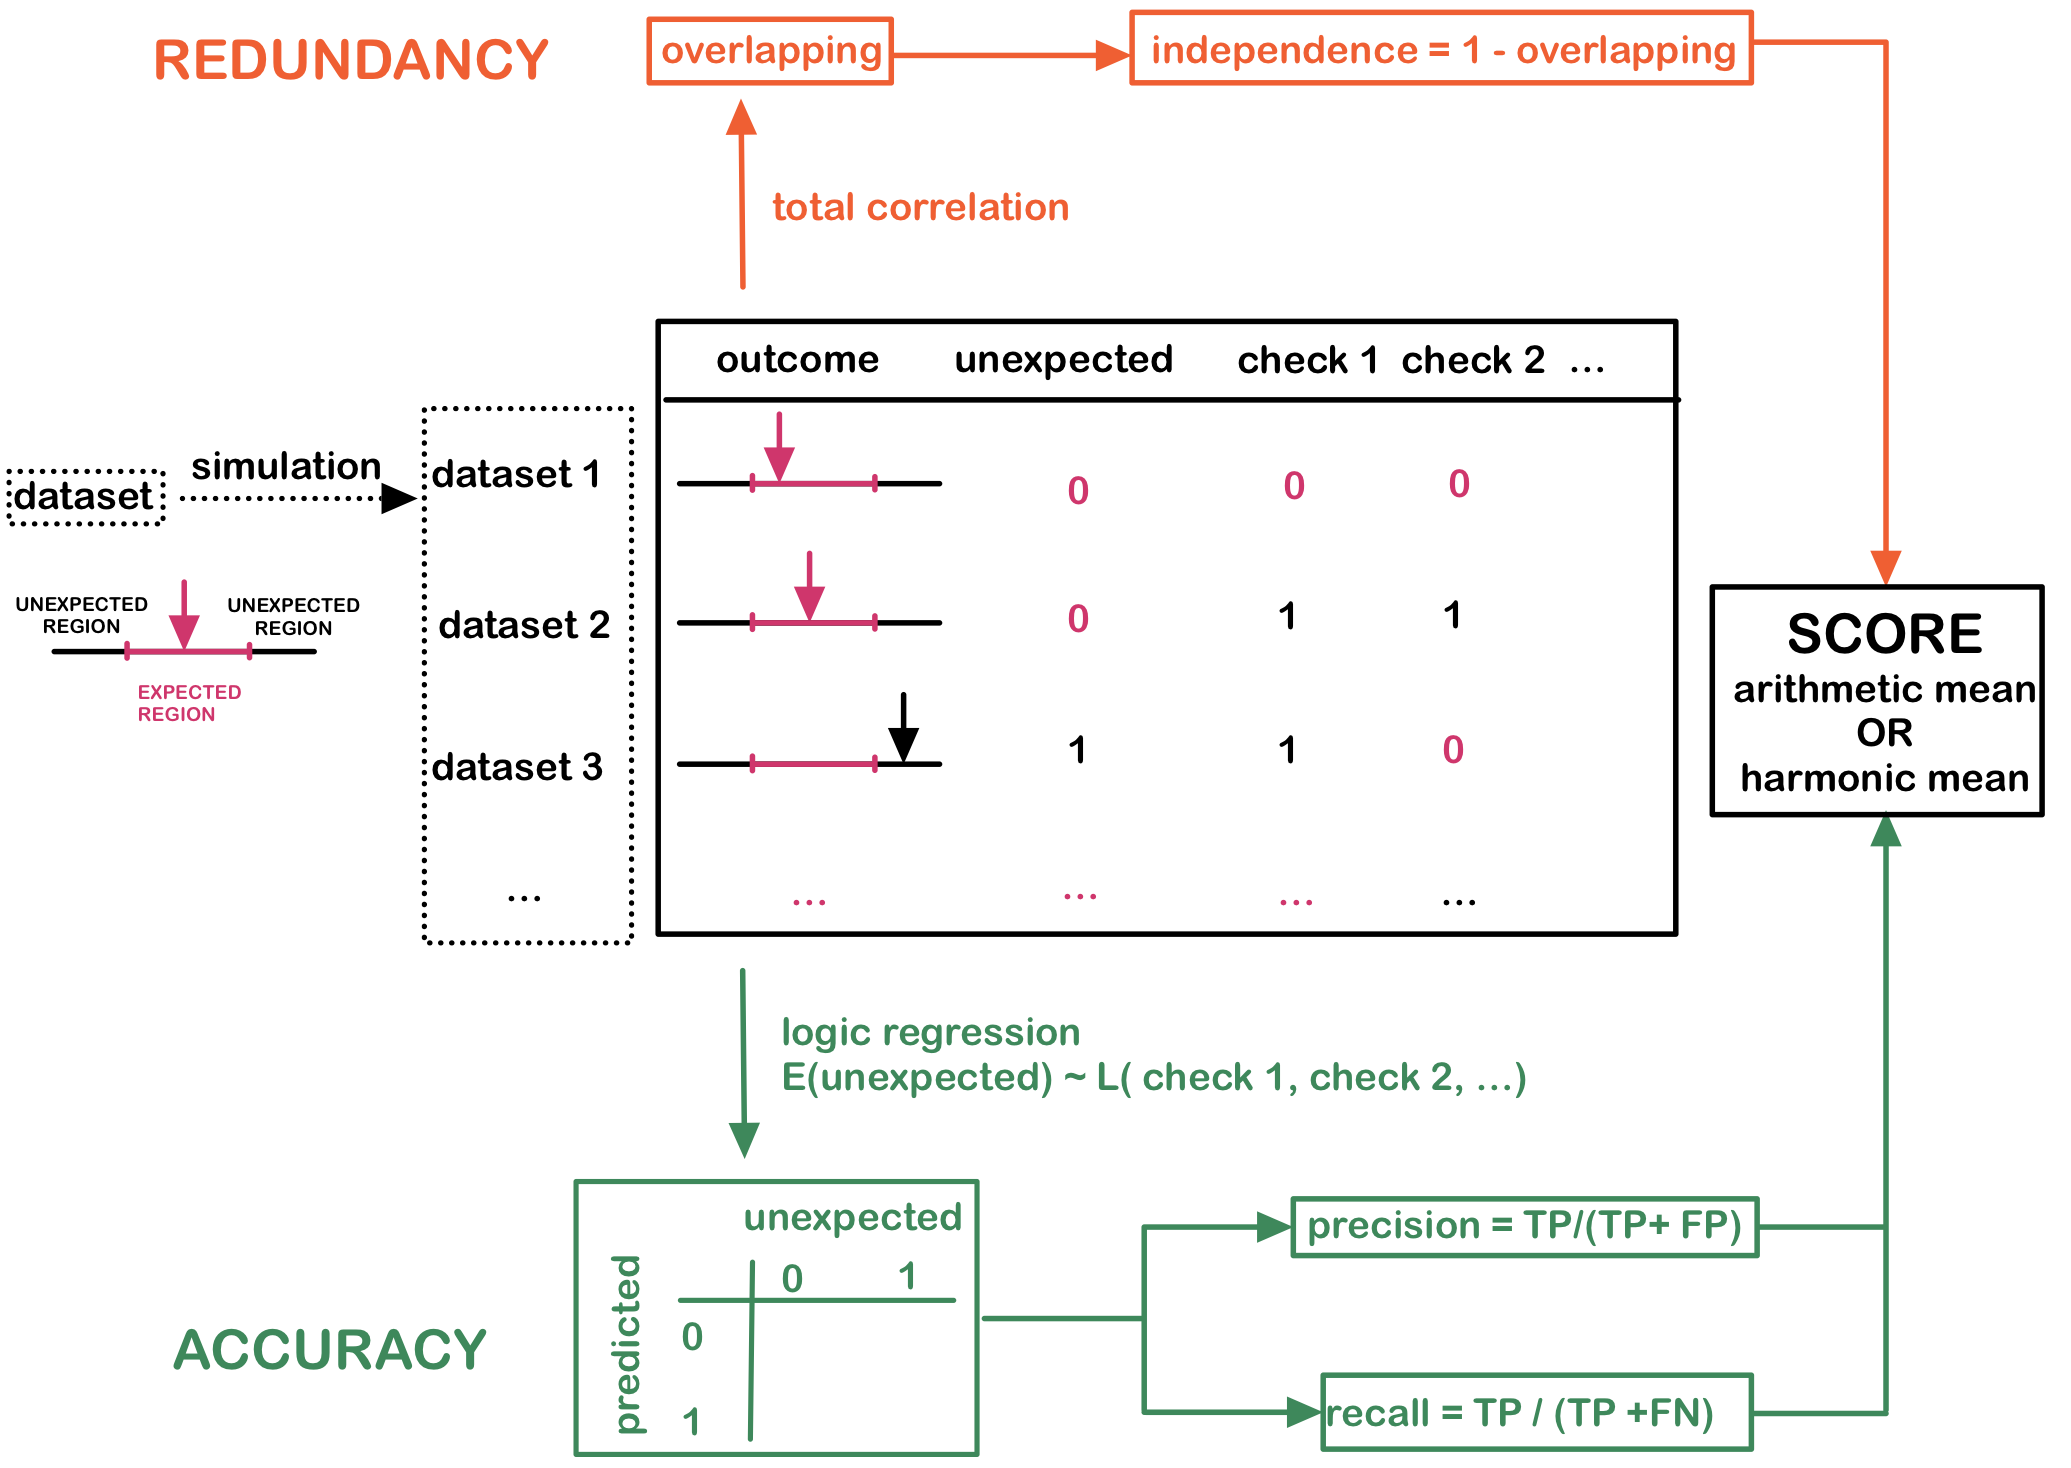
\includegraphics[width=1\linewidth,height=\textheight,keepaspectratio]{figures/metric-calc.png}

}

\caption{\label{fig-metric-calc}Overview of the procedure to quantify
the effectiveness of analysis validation checks. The procedure involves
simulating replicates of the data, applying the anlysis, and running the
analysis validation checks on each replicate to determine whether the
outcome meets the expectation (the unexpected column) and whether each
check passes (check 1, check 2, \ldots). The simulation results are then
passed to two branches: the accuracy branch calculates the precision and
recall of the checks from a logic regression prediction, while the
redundancy branch to calculate the mutual information and independence
of the checks. These three metrics are combined to produce a single
metric that quantifies the effectiveness of the checks in diagnosing
unexpected outcomes in the analysis.}

\end{figure}%

From the simulated data, the accuracy branch in
Figure~\ref{fig-metric-calc} refers to a set of checks' ability to
accurately detect unexpected outcomes while minimizing false positives
and false negatives. While a false positive can raise caution or
skepticism about the data, the presence of both false positives and
false negatives suggests that the checks are overly sensitive or lack
sensitivity to unexpected outcomes, respectively.

To incorporate the effect of multiple checks on the outcome, a logic
regression model \citep{ruczinski_logic_2003} is fitted to the analysis
validation checks. Originally developed for SNP microarray data, logic
regression constructs Boolean combinations of binary variables,
\(\mathcal{L}(X_1, X_2, \cdots, X_n)\), to predict both binary and
numerical outcomes. In our case,

\begin{itemize}
\tightlist
\item
  the outcome, \(Y\), is a binary variable indicating whether the result
  is \emph{unexpected} (1) or \emph{expected} (0),
\item
  \(X_1, X_2, \cdots, X_n\) represent the binary analysis validation
  checks, where each check is labeled as 1 if it fails and 0 if it
  passes.
\end{itemize}

For classification problems, the logic regression model is reduced to
the following form:

\[E(Y) = \mathcal{L}(X_1, X_2, \cdots, X_n)\] The logical operations of
the binary variables \(X_1, X_2, \cdots, X_n\), including AND
(\(\land\)), OR (\(\lor\)), and NOT (\(\neg\)) and an example of such
logic combination can be \(X_1 \text{ AND } (X_2 \text{ OR } X_3)\).
Simulated annealing is used to explore the search space by minimizing
the mis-classification error. The following 6 moves are permitted during
the search (as detailed in Figure 2 of \citet{ruczinski_logic_2003}): 1)
replacing a leaf node, 2) replacing an operator, 3) growing a branch, 4)
pruning a branch, 5) splitting a leaf node, and 6) deleting a leaf node.

Compared to other tree-based methods for binary-binary prediction, the
Boolean combinations from the logic regression model produce a tree
structure that can be directly interpreted as the possible combination
of checks leading to an unexpected outcome, without the need to invert
the tree as required in classic tree-based recursive partitioning
methods. The logic regression model is then used to predict the analysis
result based on the values of checks, and the prediction is compared to
the actual analysis result in order to calculate the precision and
recall of the checks.

While checks may score high on predictive accuracy, they may be less
effective at explaining the various reasons behind unexpected results.
This could happen if, for example, a set of checks are all tangentially
related to the cause of the unexpected results, but none addresses the
root cause. It may also occur if the checks are highly correlated with
one another, leading to redundancy.

To quantify redundancy, the concept of mutual information is used.
Mutual information \(I(x, y)\) measures the amount of information shared
between two random variables and is defined as the Kullback-Leibler
distance \(D(p \parallel q)\) between the joint distribution of the two
variables and the product of the marginal distributions:

\[I(x,y) = D\big(p(x,y) \parallel p(x)p(y)\big) = \sum_x \sum_y p(x,y) \log \frac{p(x,y)}{p(x)p(y)}\]

This concept extends naturally to multiple variables through total
correlation, \(C(X_1, X_2, \cdots, X_n)\), which captures redundancy
across a set of \(n\) variables:

\[C(X_1, X_2, \cdots, X_n) = \sum_{x_1} \sum_{x_2} \cdots \sum_{x_n} p(x_1, x_2, \cdots, x_n) \log \frac{p(x_1, x_2, \cdots, x_n)}{p(x_1)p(x_2) \cdots p(x_n)}\]

A high mutual information value indicates redundancy among the checks,
while a low value suggests that the checks are independent and provides
unique information to diagnose the unexpected outcome. To standardize
this measure, the total correlation \emph{per observation} is
calculated, and an independence score, ranging between 0 and 1, is
defined as 1 - mutual information.

To combine precision, recall, and independence into a single metric, we
can combine the three scores using the arithmetic mean, harmonic mean,
or quadratic mean. The differences among these means are minimal when
the three metrics are similar. However, as the differences among the
metrics increases, the harmonic mean tends to produce the smallest
overall score, as it penalizes low values, while the quadratic mean
tends to produce the largest score by rewarding higher values more. For
simple interpretation of the score, the arithmetic mean is preferred,
while in applications where the difference between precision, recall,
and independence need to be penalized or rewarded more, the harmonic and
quadratic mean should be considered.

\subsection{Toy Example Revisited}\label{toy-example-revisited}

Returning to the step count example introduced in Section~\ref{sec-toy},
the logic regression model is fitted to the three analysis checks
described previously to generate the prediction of the unexpected
outcome, whether the average number of step falls within the {[}8,500,
9,500{]} interval. The predictions from the logic regression model can
be compared with the simulated true outcome for calculating the
precision and recall metrics. Figure~\ref{fig-logic-reg} shows the
best-fitting logic regression model as

(quantile(step, 0.6) \textgreater{} 10,000 OR quantile(step, 0.4)
\textless{} 8,000) AND sd(step) \textless{} 2,500

In other words, we would predict an unexpected outcome in the analysis
if the standard deviation of the step count is not too large (2,500) and
either the 60\% quantile of the step count exceeds 10,000 or the 40\%
quantile of the step count falls below 8,000.

\phantomsection\label{cell-fig-logic-reg}
\begin{figure}[H]

\centering{

\pandocbounded{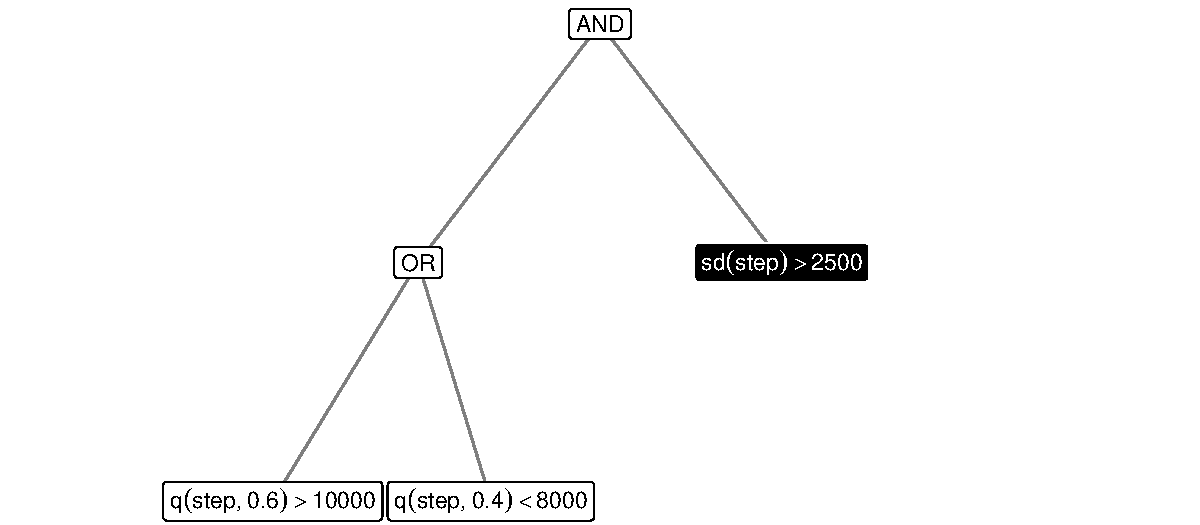
\includegraphics[keepaspectratio]{index_files/figure-pdf/fig-logic-reg-1.pdf}}

}

\caption{\label{fig-logic-reg}Logic regression model fitted to the three
checks. The model suggests the rule (quantile(step, 0.6) \textgreater{}
10,000 OR quantile(step, 0.4) \textless{} 8,000) AND (NOT sd(step)
\textgreater{} 2,500). The NOT operator applied to
\texttt{sd(step)\ \textgreater{}\ 2,500} is colored with a black
background to distinguish it from other checks.}

\end{figure}%

Table~\ref{tbl-logic-reg} presents the calculated precision, recall, and
independence for the three individual checks and the check rule found by
the logic regression. The harmonic and arithmetic means are included to
combine the three measures. The results show that the three checks
produced by the logic regression can accurately predict 86.1\% cases of
all \emph{actual unexpected results} in the simulation data.
Furthermore, 43.1\% of all \emph{predicted unexpected results} were in
fact observed to be unexpected.

\begin{table}

\caption{\label{tbl-logic-reg}Accuracy (precision and recall) and
parsimony (independence) metrics for each individual check and the logic
regression check rule. The harmonic and arithmetic means of the three
metrics are included to evaluate the quality of the checks in diagnosing
unexpected step counts (more than five days with fewer than 8,000
steps).}

\centering{

\centering
\resizebox{\ifdim\width>\linewidth\linewidth\else\width\fi}{!}{
\begin{tabular}{>{\raggedright\arraybackslash}p{17em}rrrrr}
\toprule
checks & precision & recall & indep. & harmonic & arithmetic\\
\midrule
Check 1: q(step, 0.6) > 10000 & 0.319 & 0.575 & 1.000 & 0.511 & 0.631\\
Check 2: q(step, 0.4) < 8000 & 0.264 & 0.613 & 1.000 & 0.467 & 0.626\\
Check 3: sd(step) > 2500 & 0.153 & 0.289 & 1.000 & 0.273 & 0.481\\
Logic regression: (check 1 OR check 2) AND (not check 3) & 0.861 & 0.431 & 0.998 & 0.669 & 0.763\\
Regression tree & 0.542 & 0.780 & 1.000 & 0.727 & 0.774\\
\bottomrule
\end{tabular}}

}

\end{table}%

For comparison, the regression tree produces a similar prediction to the
logic regression, however, we argue that the logic regression tree shown
in Figure~\ref{fig-logic-reg} is more interpretable for our purposes
because it provides a direct representation of which combinations of
analysis checks lead to unexpected outcomes. The logic regression tree
is also directly comparable to other diagnostic techniques, which we
discuss further in Section~\ref{sec-discussion}.

\section{Application}\label{sec-pm10-mortality}

In the study of the health effects of outdoor air pollution, one area of
interest is the association between short-term, day-to-day changes in
particulate matter air pollution and daily mortality counts. Substantial
work has been done to study this question and to date, there appears to
be strong evidence of an association between particulate matter less
than 10 \(\mu\)g/m\(^3\) in aerodynamic diameter (PM10) and daily
mortality from all non-accidental causes \citep{samet2000fine}. For our
second example, we use the problem of studying PM10 and mortality along
with data from the National Morbidity, Mortality, and Air Pollution
Study (NMMAPS) to demonstrate how our analysis validation checks
described in Section~\ref{sec-method} can be applied. The dataset that
we use to develop our simulations and analysis checks is from New York
City, and contains daily PM10, all-cause (non-accidental) mortality, and
average temperature values from 1992--2000. We then will apply the
analysis checks to similar data from 39 other cities from the NMMAPS
study.

The typical approach to studying the association between PM10 and
mortality is to apply a generalized linear model with a Poisson link to
relate daily mortality counts to daily measures of PM10. Based on
previous work and the range of effect sizes published in the literature,
an analyst might expect the coefficient for PM10 in this GLM to lie
between \([0, 0.005]\), after adjusting for daily temperature
\citep{samet2000fine, welty2005acute}. Note that the relatively simple
modeling approach being used here is primarily for demonstration;
typically far more sophisticated semi-parametric approaches are used in
the literature \citep{peng2006model}.

For the purposes of this application, observing an estimated coefficient
outside of the expected interval is considered unusual and might warrant
a re-examination of the analysis process. Therefore, our unexpected
outcome in this analysis will be the binary indicator of whether the
estimated coefficient for PM10 in the GLM lies outside of the interval
\([0, 0.005]\). In addition to providing a more substantial problem for
our methods, this example also demonstrates how the procedure presented
in Section~\ref{sec-method} can be used to select cutoff values in the
analysis checks to diagnose an unexpected PM10 coefficient from the
generalized linear model.

This PM10 coefficient expectation can be framed as an analysis check
that fails, labelled as 1, if the estimate of the PM10 coefficient
(adjusted for temperature) is outside the range {[}0, 0.005{]}, and 0 if
it is within. Multiple factors can affect the estimated PM10
coefficient, such as the strength of the correlation between mortality
and PM10, or between mortality and temperature. Outliers in the three
variables can also leverage the coefficient. While these are possible
factors that could affect the analysis result, it is not clear what the
cutoff values for these checks should be to determine a failure. Here we
consider a list of checks in Table~\ref{tbl-checks} with varied cutoff
values for each:

\begin{longtable}[]{@{}l@{}}
\caption{A list of checks considered for the generalized linear model of
mortality on PM10 and temperature. The checks are based on the sample
size, correlation between mortality and PM10, correlation between
mortality and temperature, and univariate outlier detection. Multiple
cutoff values are specified for each check to determine a
failure.}\label{tbl-checks}\tabularnewline
\toprule\noalign{}
The check fails (encoded as 1) if \ldots{} \\
\midrule\noalign{}
\endfirsthead
\toprule\noalign{}
The check fails (encoded as 1) if \ldots{} \\
\midrule\noalign{}
\endhead
\bottomrule\noalign{}
\endlastfoot
Mortality-PM10 correlation less than \(-0.05\) \\
Mortality-PM10 correlation less than \(-0.03\) \\
Mortality-PM10 correlation greater than \(0.03\) \\
Mortality-PM10 correlation greater than \(0.05\) \\
Mortality-temperature correlation greater than \(-0.3\) \\
Mortality-temperature correlation greater than \(-0.35\) \\
Mortality-temperature correlation greater than \(-0.4\) \\
Mortality-temperature correlation greater than \(-0.45\) \\
Outlier(s) are presented in the variable PM10 \\
Outlier(s) are presented in the variable mortality \\
\end{longtable}

\subsection{Data Simulation}\label{data-simulation}

To generate replicates of the dataset, we first generate the correlation
matrix of the three variables (PM10, mortality, and temperature) in a
grid and then use a Gaussian copula to generate a multivariate normal
distribution based on the specified correlation matrix and sample size.
The multivariate normal distribution is transformed using the normal CDF
before the inverse CDF of the assumed distributions of the three
variables is applied. To determine the appropriate distribution of each
variable, various distributions are fitted and compared. This includes
poisson and negative binomial for mortality; gamma, log-normal,
exponential, weibull, and normal for PM10 and temperature; and beta for
PM10 after rescaling the data to \([0,1]\).

To ensure a reasonable likeness to data that might be used in such an
analysis, we use characteristics of the observed New York City dataset
to refine our simulations. AIC is used to determine the best
distribution fit for each variable with the QQ-plot presented in
Figure~\ref{fig-dist-fit} to evaluate the fit. AIC suggests a negative
binomial distribution for mortality, a beta distribution for PM10
(multiple by 100 to recover the original scale), and a Weibull
distribution for temperature. To include the potential effect of
outliers, we add a single outlier to the data for both the mortality and
PM10 variables.

\phantomsection\label{cell-fig-dist-fit}
\begin{figure}[H]

\centering{

\pandocbounded{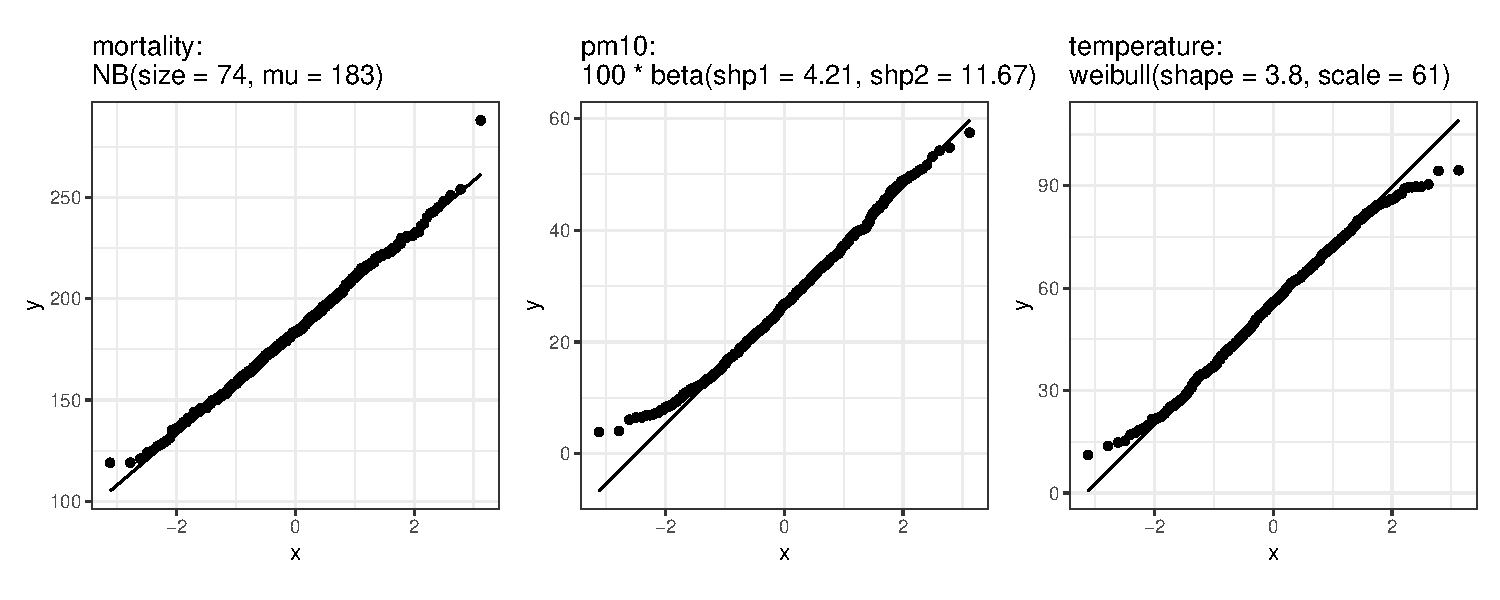
\includegraphics[keepaspectratio]{index_files/figure-pdf/fig-dist-fit-1.pdf}}

}

\caption{\label{fig-dist-fit}QQ-plot of the distribution fit for
mortality, PM10, and temperature based on the fitted distribution from
the original data. The fitted distribution is compared to the observed
data to assess the distribution fit.}

\end{figure}%

A logic regression is fitted using all variations of the checks in
Table~\ref{tbl-checks} to predict whether the PM10 coefficient is
unexpected. Given the imbalance of outcome (expected vs.~unexpected),
inverse weights proportional to the number of observations in each
outcome are applied during the logic regression fit.
Figure~\ref{fig-linear-reg-tree} shows the optimal logic regression tree
from the fitted model. Precision, recall, and independence score, along
with their harmonic and arithmetic mean are calculated in
Table~\ref{tbl-linear-reg}.

\begin{figure}

\centering{

\pandocbounded{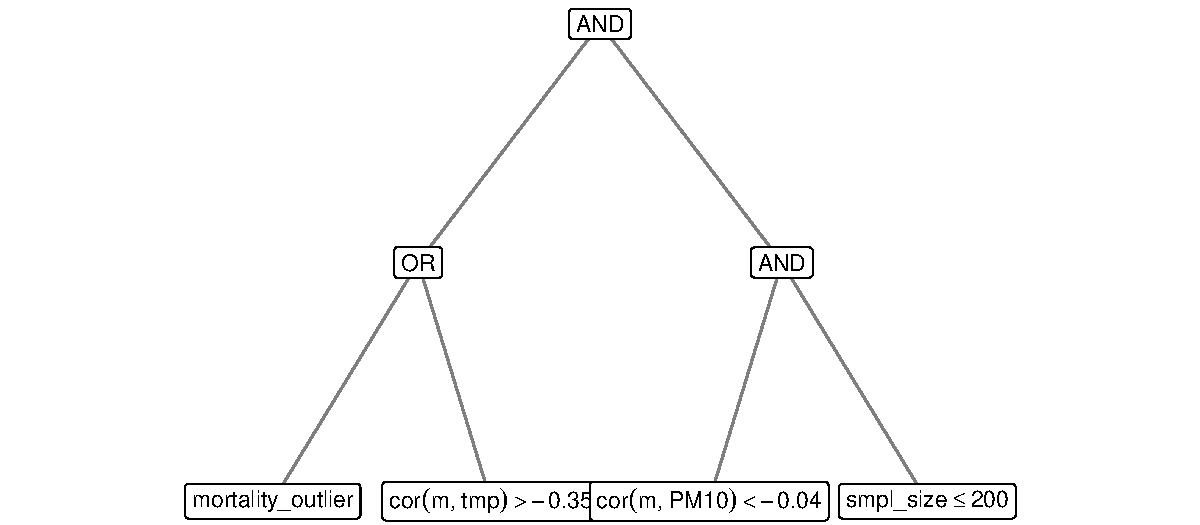
\includegraphics[keepaspectratio]{index_files/figure-pdf/unnamed-chunk-8-1.pdf}}

}

\caption{\label{fig-linear-reg-tree}Logic regression model fitted to the
fourteen checks and the outcome expectation (unexpected) as the response
variable. The model suggests the relationship: (mortality-PM10
correlation \textless{} -0.03) AND (mortality-temperature correlation
\textgreater{} -0.3 OR (there exist mortality outlier AND there exist
PM10 outlier)) to predict the unexpected PM10 coefficient.}

\end{figure}%

\begin{table}

\caption{\label{tbl-linear-reg}Accuracy (precision and recall) and
parsimony (independence) metrics derived from the logic regression model
(last row) and individual checks, along with harmonic and arithmetic
means.}

\centering{

\centering
\resizebox{\ifdim\width>\linewidth\linewidth\else\width\fi}{!}{
\begin{tabular}{>{\raggedright\arraybackslash}p{18em}rrrrr}
\toprule
check & precision & recall & indep. & harmonic & arithmetic\\
\midrule
Check 1: cor(m, PM10) < -0.03 & 0.551 & 0.894 & 1 & 0.763 & 0.815\\
Check 2: cor(m, tmp) > -0.35 & 0.281 & 0.556 & 1 & 0.472 & 0.612\\
Check 3: mortality outlier & 0.302 & 0.775 & 1 & 0.536 & 0.692\\
Check 4: PM10 outlier & 0.305 & 0.766 & 1 & 0.537 & 0.690\\
Logic regression: (check 1) AND ((check 2) OR (check 3 AND check 4)) & 0.722 & 0.876 & 1 & 0.851 & 0.866\\
\bottomrule
\end{tabular}}

}

\end{table}%

As indicated in Figure~\ref{fig-linear-reg-tree}, the logic regression
model picks up the following cutoff values for each type of check:

\begin{itemize}
\tightlist
\item
  mortality-PM10 correlation less than \(-0.03\)
\item
  mortality-temperature correlation greater than \(-0.3\)
\item
  PM10 data contains outliers that are detected by the univariate
  outlier detection
\item
  mortality data contains outliers that are detected by the univariate
  outlier detection
\end{itemize}

The tree structure suggests checking mortality-PM10 correlation and a
sample size larger than 200 with an additional check of either outlier
on mortality or correlation between mortality and temperature. This
combined check rule generates a precision of 0.722 and a recall of 0.876
for predicting the unexpected PM10 coefficient.

As shown in Figure~\ref{fig-linear-reg-tree}, there is no single
analysis check in the tree that predicts an unexpected outcome. rather
at least three checks in the tree must be TRUE in order for the model to
predict an unexpected outcome. Given the high independence of the checks
(Table~\ref{tbl-linear-reg}), this suggests that unexpected results are
only likely after multiple anomalies are observed in the data.

\subsection{Additional Cities}\label{additional-cities}

In order to test our development of analysis validation checks based on
the New York City data, we incorporate data from 39 additional cities
from the original NMMAPS study and apply our checks to those data. These
cities (along with New York City) represent approximately the largest 40
metropolitan areas in the United States by population. The complete list
of cities used are presented in Table~\ref{tbl-all-cities}. For each
city, we had daily data on all-cause mortality, PM10, and average
temperature for the years 1992--2000.

\begin{table}

\caption{\label{tbl-all-cities}Results from full analysis of 40 cities
from the NMMAPS air pollution and mortality study. In the table, a ``T''
indicates that a check failed and an ``F'' indicates that a check
passed.}

\centering{

\centering
\resizebox{\ifdim\width>\linewidth\linewidth\else\width\fi}{!}{
\begin{tabular}{lrccrrcc}
\toprule
City & \makecell[l]{PM10\\Estimated\\Coefficient} & \makecell[l]{Outcome\\Observed\\Unexpected} & \makecell[l]{Logic Regression\\Predicted\\Unexpected} & \makecell[l]{Correlation:\\Mortality-\\Temperature} & \makecell[l]{Correlation:\\Mortality-\\PM10} & \makecell[l]{Mortality\\Outlier} & \makecell[l]{PM10\\Outlier}\\
\midrule
Atlanta & -0.0008 & T & T & --0.26 (T) & --0.16 (T) & F & F\\
Austin & -0.0030 & T & T & --0.12 (T) & --0.11 (T) & F & T\\
Baltimore & 0.0018 & F & F & --0.21 (T) & 0.01 (F) & T & T\\
Boston & 0.0019 & F & F & --0.16 (T) & 0.02 (F) & F & T\\
Buffalo & 0.0028 & F & F & --0.23 (T) & --0.02 (F) & F & T\\
\addlinespace
Chicago & 0.0011 & F & F & --0.38 (F) & --0.02 (F) & T & T\\
Cincinnati & 0.0011 & F & T & --0.27 (T) & --0.06 (T) & T & T\\
Cleveland & 0.0010 & F & F & --0.30 (F) & --0.02 (F) & T & T\\
Columbus & 0.0004 & F & T & --0.20 (T) & --0.07 (T) & F & T\\
Denver & 0.0010 & F & F & --0.23 (T) & 0.06 (F) & F & T\\
\addlinespace
Detroit & 0.0011 & F & F & --0.30 (T) & 0.04 (F) & F & T\\
Dallas/Fort Worth & 0.0016 & F & T & --0.30 (F) & --0.03 (T) & T & T\\
Honolulu & 0.0006 & F & F & --0.17 (T) & 0.05 (F) & T & T\\
Houston & 0.0007 & F & F & --0.22 (T) & --0.03 (F) & F & T\\
Indianapolis & 0.0014 & F & F & --0.13 (T) & 0.02 (F) & F & T\\
\addlinespace
Kansas City & 0.0022 & F & F & --0.20 (T) & 0.02 (F) & F & T\\
Los Angeles & 0.0011 & F & F & --0.47 (F) & --0.01 (F) & T & T\\
Las Vegas & 0.0008 & F & F & --0.27 (T) & 0.05 (F) & T & T\\
Memphis & -0.0007 & T & T & --0.16 (T) & --0.10 (T) & F & T\\
Miami & -0.0004 & T & F & --0.16 (T) & --0.02 (F) & F & T\\
\addlinespace
Milwaukee & 0.0026 & F & F & --0.22 (T) & 0.09 (F) & F & T\\
Minneapolis/St. Paul & 0.0009 & F & F & --0.30 (F) & --0.01 (F) & T & T\\
New York & 0.0022 & F & F & --0.46 (F) & --0.01 (F) & T & T\\
Oakland & 0.0008 & F & F & --0.28 (T) & 0.04 (F) & F & T\\
Orlando & -0.0008 & T & T & --0.21 (T) & --0.05 (T) & F & T\\
\addlinespace
Philadelphia & 0.0021 & F & F & --0.27 (T) & 0.11 (F) & T & T\\
Phoenix & 0.0009 & F & F & --0.44 (F) & 0.07 (F) & T & T\\
Pittsburgh & 0.0009 & F & T & --0.36 (F) & --0.08 (T) & T & T\\
Riverside & 0.0001 & F & T & --0.27 (T) & --0.11 (T) & T & T\\
Sacramento & 0.0005 & F & F & --0.30 (T) & 0.05 (F) & T & T\\
\addlinespace
Salt Lake City & -0.0004 & T & T & --0.19 (T) & --0.03 (T) & F & T\\
San Antonio & -0.0021 & T & T & --0.22 (T) & --0.16 (T) & F & T\\
San Bernardino & 0.0006 & F & T & --0.28 (T) & --0.09 (T) & T & T\\
San Diego & 0.0011 & F & F & --0.33 (F) & 0.03 (F) & T & T\\
San Jose & 0.0006 & F & F & --0.23 (T) & 0.08 (F) & F & T\\
\addlinespace
Seattle & 0.0003 & F & F & --0.24 (T) & 0.06 (F) & F & T\\
Santa Ana/Anaheim & 0.0005 & F & T & --0.26 (T) & --0.04 (T) & T & T\\
St. Petersburg & 0.0012 & F & F & --0.31 (F) & 0.01 (F) & F & T\\
Tampa & -0.0003 & T & T & --0.20 (T) & --0.04 (T) & F & T\\
Tucson & 0.0028 & F & F & --0.31 (F) & 0.18 (F) & T & T\\
\bottomrule
\end{tabular}}

}

\end{table}%

We applied each of the analysis validation checks and the fitted logic
regression model separately to each of the cities' data to make
predictions of whether the outcome will be unexpected or not. We also
applied the generalized linear model to the data from each of the cities
to estimate the association between PM10 and mortality in each city,
adjusted for temperature. The estimates of the association and the
results of each of the analysis validation checks for each city are
shown in Table~\ref{tbl-all-cities}.

\begin{table}

\caption{\label{tbl-accuracy}Summary of the observed and the predicted
unexpected PM10 coefficient results from the 40 NMMAPS cities using the
logic regression model.}

\centering{

\begin{tabular}{lrr}
\toprule
\multicolumn{1}{c}{} & \multicolumn{2}{c}{Predicted} \\
\cmidrule(l{3pt}r{3pt}){2-3}
Observed & FALSE & TRUE\\
\midrule
FALSE & 25 & 7\\
TRUE & 1 & 7\\
\bottomrule
\end{tabular}

}

\end{table}%

It is clear from Table~\ref{tbl-all-cities} that some of the estimated
PM10 coefficients are outside the expected range of {[}0, 0.005{]}.
Eight of the 40 cities had negative estimated coefficients and were
therefore considered unexpected by our original criterion. (It is
perhaps worth noting that none of the unexpected outcomes was in the
positive direction.) Table~\ref{tbl-accuracy} summarizes the prediction
accuracy of the logic regression model for the 40 cities. The model
correctly predicts the PM10 coefficient status of 32 cities, producing
an accuracy rate of 80\%. Among the 8 cities with an unexpected outcome
(PM10 coefficient outside {[}0, 0.005{]}), the model correctly
identifies 7 (Atlanta, Austin, Memphis, Orlando, Salt Lake City, San
Antonio, Tampa), giving a recall of 88\% (only Miami was not properly
classified by the logic regression model). These cities were flagged due
to failures in both the mortality-PM10 correlation and
mortality-temperature correlation analysis checks. Out of the 14 cities
with positive predictions from the model, 7 cities (Cincinnati,
Columbus, Dallas/Fort Worth, Pittsburgh, Riverside, San Bernardino,
Santa Ana/Anaheim) were false positives, resulting in a precision of
only 50\%. This precision value is substantially lower than what was
estimated by the simulation procedure (see Table~\ref{tbl-linear-reg})
and suggests that the simulation does not adequately capture some
features of the data generation process.

\section{Discussion}\label{sec-discussion}

In this paper we have developed an approach to using analysis validation
checks to externalize the assumptions about the data and analysis tools
made during the data analysis process. These checks can serve as a
useful summary of the analyst's thought process and can describe how
characteristics of the data may lead to unexpected outcomes. Using logic
regression, we can develop a graphical summary of the analysis
validation checks as well as use the logic regression fitting process to
choose the optimal set of checks. The logic regression model can also be
used to develop summaries of the precision and recall of the collection
of analysis validation checks in predicting the likelihood of an
unexpected outcome. We demonstrated our method on an example relating
daily mortality to outdoor air pollution data. The results from that
example could be used to inform future analyses of air pollution and
health data, perhaps in other cities or locations.

With the analysis validation checks proposed in this paper, analysts may
perform these checks \emph{ex ante} to identify and address potential
issues before proceeding with the analysis or use them \emph{ex post} to
diagnose the analysis when an unexpected outcome occurs. Theses checks
act as checkpoints designed by analysts to flag potential issues,
clarify assumptions made during the analysis, and enhance transparency
and communication among stakeholders. They also support students and
junior researchers develop the skills needed to independently diagnose
issues in analyses.

In Section~\ref{sec-pm10-mortality} we used the analysis checks in a
diagnostic manner to examine the eight cities whose PM10 coefficients
were unexpected. There, we found that seven of the cities had a
mortality-PM10 correlation that was more negative than expected while
also having a mortality-temperature correlation that was somewhat larger
(less negative) than expected. What this result implies for the broader
analysis depends on a number of factors, but the interplay between
mortality, PM10, and temperature may warrant further investigation
\citep[see e.g.][]{welty2005acute}. Note that simply because the PM10
coefficient estimates were unexpected by our criterion, we do not mean
to imply that they are ``wrong'' in any sense. Indeed, negative
estimated coefficients have been found in other studies of this nature
\citep{bell2004ozone}. Rather, in this type of analysis, it may be that
the interval for expected results needs to be revised. Further, it may
be necessary to incorporate other outputs from the analysis, such as
measures of uncertainty.

An interesting connection can be drawn between our logic regression
trees and a tool used in systems engineering known as a fault tree. A
fault tree is used for conducting a structured risk assessment and has a
long history in aviation, aerospace, and nuclear power applications
\citep{vesely1981fault}. A fault tree is a graphical tool that describes
the possible combinations of causes and effects that lead to an anomaly.
At the top of the tree is a description of an anomaly. The subsequent
branches of the tree below the top event indicate possible causes of the
event immediately above it in the tree. The tree can then be built
recursively until we reach a root cause that cannot be further
investigated. Each level of the tree is connected together using logic
gates such as AND and OR gates. The leaf nodes of the tree indicate the
root causes that may lead to an anomaly. While the logic regression
tress are not identical to fault trees, they share many properties, such
as the tree-based structure and the indicator of root causes at the leaf
nodes. Perhaps more critically, both serve as graphical summaries of the
assumptions made in a problem and the specific violations of those
assumptions that could lead to an unexpected result. While fault trees
are often used to discover the root cause of an anomaly after it occurs,
an important use case for fault trees is to develop a comprehensive
understanding of a system \emph{before} an anomaly occurs
\citep{michael2002fault}.

Visualization methods are also valuable tools for assessing data
assumptions and can potentially be formalized as analysis validation
checks. For instance, plotting a variable's distribution using a
histogram, density plot, or bee swarm plot can reveal outliers or
deviations from normality. These visualizations could be re-framed as
checks that fail when the data does not conform to the expected
distribution. However, translating visualization results into binary
checks that return (TRUE, FALSE) remains an open challenge, requiring
either manual verification or the development of automated methods to
interpret visualization outputs. An existing example of visual test is
the R package \texttt{vdiffr} \citep{vdiffr} for software unit testing.
The package saves a template plot and compares it to the current plot to
determine whether the unit tests passes or fails.

Systematically generating realistic simulated data is a key component of
our approach and is deserving of further consideration. In the PM10
example in Section~\ref{sec-pm10-mortality}, the inverse transform
method was used to preserve the correlation structure among mortality,
PM10, and temperature. However, the simulation process can become
complex when additional restrictions are imposed or when a greater range
of scenarios is desired. In such cases, techniques like the
acceptance-reject method or permutation may be used to generate the
data. The results in Section~\ref{sec-pm10-mortality} on the broader
NMMAPS dataset suggest that our simulation procedure may have been
inadequate in reflecting the range of possible configurations that the
data could take. In particular, our split-data approach, using New York
City to guide the simulation and then applying the analysis checks to
other cities, may not have been ideal. It may be worth exploring some
recent work in data thinning \citep{neufeld2024data} and data fission
\citep{leiner2023data} to create training datasets that are more
representative of future data.

Analysis validation checks are closely related to the concept of unit
testing in software engineering. While unit tests isolate and test
specific lines of the code, analysis validation checks focus on the
assumptions underlying the analysis rather than the explicit code
itself. Moreover, while software testing is deterministic, with clear
rules for determining failure, analysis validation checks are
probabilistic. As a result, an analysis may fail several assumption
checks yet produce an expected outcome, or pass all checks but yield an
unexpected result.

Communicating the process of data analysis is a key element to providing
transparency, improving reproducibility, and building trust with a range
of audiences. The analysis validation checks described here provide a
general way to encode the assumptions that an data analyst makes about
the data and statistical tools applied to the data. These assumptions
can be studied or challenged, depending on the specific analyst's
perspective, and can serve as a roadmap for diagnosing unexpected
results.

\section{Acknowledgement}\label{acknowledgement}

The article is created using Quarto \citep{Allaire_Quarto_2022} in R
\citep{R}. The source code for reproducing the work reported in this
paper can be found at:
\url{https://github.com/huizezhang-sherry/paper-avc}.


\renewcommand\refname{References}
  \bibliography{references.bib}



\end{document}
